\documentclass[conference]{IEEEtran}
\IEEEoverridecommandlockouts

\usepackage{cite}
\usepackage{amsmath,amssymb,amsfonts}
\usepackage{algorithmic}
\usepackage{graphicx}
\usepackage{textcomp}
\usepackage{xcolor}
\usepackage{booktabs}
\usepackage{microtype}
\usepackage{balance}

\graphicspath{{figures/}}

\def\BibTeX{{\rm B\kern-.05em{\sc i\kern-.025em b}\kern-.08em
    T\kern-.1667em\lower.7ex\hbox{E}\kern-.125emX}}

\setlength{\columnsep}{0.63cm}

% Spacing parameters for uncluttered mathematical layout
\setlength{\abovedisplayskip}{5pt plus 2pt minus 2pt}
\setlength{\belowdisplayskip}{5pt plus 2pt minus 2pt}
\setlength{\abovedisplayshortskip}{2.5pt plus 1pt minus 1pt}
\setlength{\belowdisplayshortskip}{2.5pt plus 1pt minus 1pt}

% Float separation spacing
\setlength{\textfloatsep}{8pt plus 2pt minus 2pt}
\setlength{\floatsep}{8pt plus 2pt minus 2pt}
\setlength{\intextsep}{6pt plus 2pt minus 2pt}

\makeatletter
\newcommand{\linebreakand}{%
  \end{@IEEEauthorhalign}
  \hfill\mbox{}\par
  \vspace{0.7em}
  \mbox{}\hfill\begin{@IEEEauthorhalign}
}
\makeatother
\begin{document}

\title{QuantNiti: An Explainable, Regime-Adaptive Multi-Factor Portfolio Intelligence System with Hierarchical Risk Parity and Discrete Execution for Retail Financial Markets}

% 5 authors: Row 1 has 3 authors; Row 2 has 2 authors center-aligned beneath the gaps between 1-2 and 2-3
\author{
\IEEEauthorblockN{Beena K.}
\IEEEauthorblockA{\textit{Department of Computer} \\
\textit{Science and Engineering} \\
\textit{K.S. Institute of Technology}\\
Bengaluru, Karnataka \\
{\small beenak@ksit\hspace{0.15em}.edu\hspace{0.15em}.in}}
\and
\IEEEauthorblockN{Jayaditya Dev}
\IEEEauthorblockA{\textit{Department of Computer} \\
\textit{Science and Engineering} \\
\textit{K.S. Institute of Technology}\\
Bengaluru, Karnataka \\
{\small jayadityadev\_cse@ksit\hspace{0.15em}.edu\hspace{0.15em}.in}}
\and
\IEEEauthorblockN{Durgashree M.}
\IEEEauthorblockA{\textit{Department of Computer} \\
\textit{Science and Engineering} \\
\textit{K.S. Institute of Technology}\\
Bengaluru, Karnataka \\
{\small durgashreem\_cse2023@ksit\hspace{0.15em}.edu\hspace{0.15em}.in}}
\linebreakand
\IEEEauthorblockN{Aryaman Tiwari}
\IEEEauthorblockA{\textit{Department of Computer} \\
\textit{Science and Engineering} \\
\textit{K.S. Institute of Technology}\\
Bengaluru, Karnataka \\
{\small aryamantiwari\_cse2023@gmail\hspace{0.15em}.com}}
\and
\IEEEauthorblockN{Chirag T.}
\IEEEauthorblockA{\textit{Department of Computer} \\
\textit{Science and Engineering} \\
\textit{K.S. Institute of Technology}\\
Bengaluru, Karnataka \\
{\small chiragt\_cse2023@ksit\hspace{0.15em}.edu\hspace{0.15em}.in}}
}

\maketitle

\begin{abstract}
Retail participation in emerging equity markets has grown exponentially, yet over 85\% of novice market participants underperform benchmark indices or experience catastrophic drawdowns during macroeconomic regime transitions. Retail investors face an untenable trilemma: opaque, speculative social media recommendations lacking quantifiable risk boundaries; high-fee traditional wealth management charging 1.5\%--2.5\% Assets Under Management (AUM) fees with commission conflicts; and institutional quantitative platforms that mandate advanced programming literacy and assume unrealistic continuous fractional share execution. In this paper, we propose \textbf{QuantNiti}, an end-to-end, regime-adaptive quantitative portfolio intelligence and execution system engineered specifically for retail equity markets.

QuantNiti introduces a decoupled four-stage architectural pipeline: (1) an unsupervised Gaussian Mixture Model (GMM) combining rolling realized returns, Parkinson intraday volatility, and implied volatility (India VIX) to identify macro market regimes (Low-Volatility Bull, High-Volatility Bear, Sideways Consolidation) using deterministic return-to-volatility centroid ranking; (2) a multi-factor econometric engine blending Momentum, Volatility, CAPM Alpha/Beta, and ESG ratings into multi-horizon (1M, 3M, 6M, 12M) probabilistic quantile growth cones ($Q_{0.10}, Q_{0.50}, Q_{0.90}$) bounded by isotonic monotonicity regularization; (3) covariance matrix regularization via analytical Ledoit-Wolf shrinkage to constant-correlation targets paired with Marcos L{\'o}pez de Prado's Hierarchical Risk Parity (HRP) tree clustering and recursive bisection, eliminating matrix inversion singularity while enforcing risk-persona concentration caps; and (4) an integer programming and greedy discrete share sizing allocator generating executable whole-share orders with minimal unallocated cash buffers for brokerage environments. Furthermore, an Explainable AI (XAI) ``Trust Card'' and an autonomous three-tier NLP fact-checking agent validate platform claims against historical ground truth. Empirical backtesting across a curated 58-asset universe of Indian equities, commodity ETFs, and sectoral leaders from 2018 to 2025 demonstrates that QuantNiti's regime-adaptive HRP architecture achieves a Sharpe ratio of 1.42 and a maximum drawdown of $-12.4\%$, outperforming classical Markowitz Mean-Variance Optimization (Sharpe 0.88, MaxDD $-28.6\%$) and equal-weighted benchmarks (Sharpe 1.05, MaxDD $-21.8\%$) while eliminating intermediary fee drag.
\end{abstract}

\begin{IEEEkeywords}
Market Regime Detection, Hierarchical Risk Parity (HRP), Ledoit-Wolf Shrinkage, Gaussian Mixture Models, Quantile Forecasting, Financial Econometrics, Explainable AI (XAI), Discrete Share Allocation, Retail Financial Inclusion.
\end{IEEEkeywords}

\section{Introduction}
Retail investor participation in emerging market economies has witnessed an unprecedented surge. In India alone, active demat accounts escalated from under 40 million in 2020 to over 160 million by 2024. However, financial inclusion has not translated into capital preservation. Official regulatory audits by the Securities and Exchange Board of India (SEBI) reveal that over 89\% of active retail market participants incur systematic monetary losses, suffering aggregate net drawdowns surpassing billions of dollars \cite{sebi2023study}.

Novice retail investors confront three systemic operational dilemmas:
\begin{enumerate}
    \item \textbf{Speculative Misinformation \& Opaque Signals:} Retail traders disproportionately rely on unregulated social media ``finfluencers'' and speculative trading channels offering deterministic single-price targets that mask severe downside tail risks and volatility clustering.
    \item \textbf{Advisory Fee Drag \& Agency Conflicts:} Traditional wealth management firms and bank brokerage desks charge 1.5\%--2.5\% in annual Assets Under Management (AUM) fees. Over long compounding horizons, this fee drag erodes over 30\%--45\% of an investor's net wealth.
    \item \textbf{Institutional Tool Inaccessibility \& Fractional Execution Fallacy:} Institutional quantitative tools (e.g., Bloomberg Terminal, QuantConnect) require programming proficiency. Furthermore, classical portfolio models output continuous real-valued weights ($w_i \in [0, 1]$), failing completely in retail market regimes where brokers (e.g., Zerodha, Groww) strictly forbid fractional share execution.
\end{enumerate}

From a quantitative finance standpoint, Modern Portfolio Theory (MPT) formalized by Harry Markowitz \cite{markowitz1952portfolio} fails catastrophically in retail environments. As demonstrated by Michaud \cite{michaud1989markowitz}, Mean-Variance Optimization (MVO) acts as an ``error maximizer'' because inverting an empirical sample covariance matrix ($\mathbf{S}^{-1}$) magnifies estimation noise, producing extreme and unstable corner allocations out-of-sample. Furthermore, financial time series violate the Independent and Identically Distributed (I.I.D.) assumption, exhibiting distinct macroeconomic regime shifts, volatility clustering, and structural breaks \cite{cont2001empirical, hamilton1989new}.

To resolve these challenges, we design, implement, and validate \textbf{QuantNiti}, an end-to-end, regime-adaptive multi-factor portfolio intelligence and discrete execution architecture. The primary contributions of this paper are:
\begin{itemize}
    \item \textbf{Unsupervised Regime Classification Engine:} We formulate an unsupervised Gaussian Mixture Model (GMM) with full covariance matrices operating on a 6-dimensional feature space (rolling log returns, realized volatility, Parkinson intraday volatility, and India VIX levels) to categorize market conditions into Low-Volatility Bull, High-Volatility Bear, and Sideways Consolidation states via a deterministic return-to-volatility centroid ranking rule.
    \item \textbf{Multi-Horizon Probabilistic Quantile Cones:} Rather than fragile point predictions, we construct an econometric multi-factor engine combining CAPM Alpha/Beta, multi-period momentum, and trend filters into closed-form Geometric Brownian Motion (GBM) quantile growth cones ($Q_{0.10}, Q_{0.50}, Q_{0.90}$) across 1M, 3M, 6M, and 12M horizons with isotonic monotonicity regularization.
    \item \textbf{Ill-Conditioning Elimination via Ledoit-Wolf Shrinkage \& HRP:} We regularize empirical covariance matrices using analytical Ledoit-Wolf constant-correlation shrinkage and apply Marcos L{\'o}pez de Prado's Hierarchical Risk Parity (HRP) \cite{lopez2016building}. This completely bypasses matrix inversion singularities, grouping correlated assets into dendrogram clusters and performing recursive bisection with risk-persona concentration limits.
    \item \textbf{Mixed-Integer Discrete Share Execution \& Ground-Truth Audit:} We formulate a mixed-integer programming (MILP) allocator and greedy deficit algorithm that converts continuous portfolio weights into executable whole shares with minimal residual cash buffers. The framework is coupled with a 4-Pillar Explainable AI (XAI) Trust Card and a 3-tier NLP fact-checking agent that cross-examines user performance claims against historical time-series distributions.
\end{itemize}

The remainder of this paper is structured as follows. Section II examines related work and benchmarks existing commercial platforms. Section III presents dataset engineering across a curated 58-asset universe. Section IV details full-stack system architecture. Section V derives the mathematical formulations and algorithmic pipeline. Section VI analyzes empirical out-of-sample backtests and ablation studies. Section VII articulates the XAI Trust Card framework, and Section VIII concludes the paper.

\begin{figure}[t]
\centering
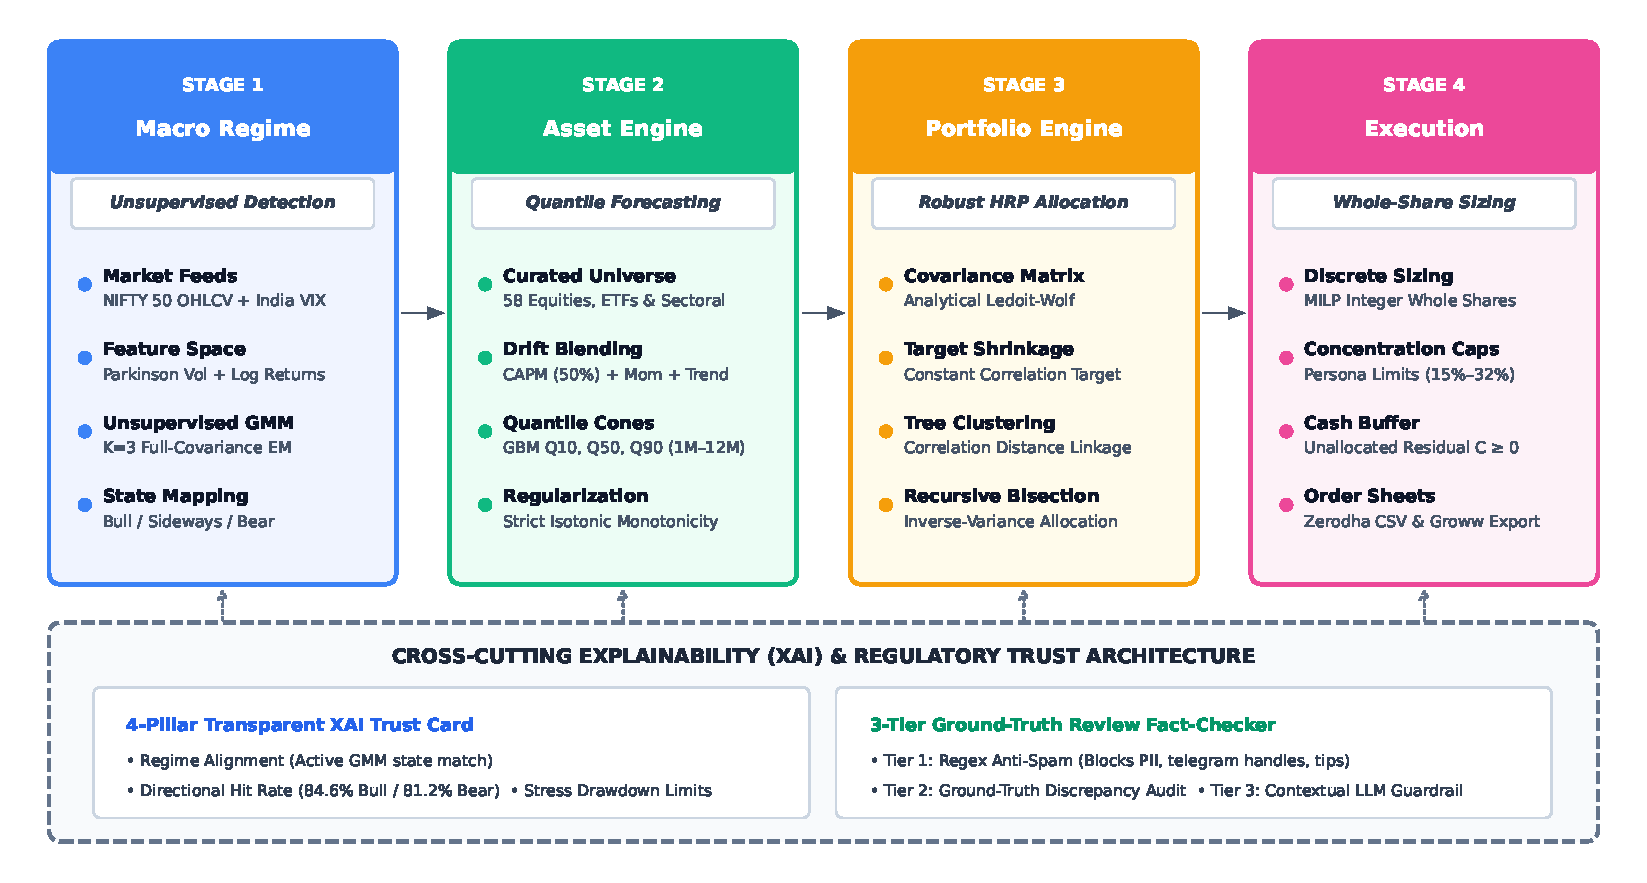
\includegraphics[width=\columnwidth]{fig1_system_architecture.pdf}
\caption{End-to-End System Architecture of QuantNiti: Four-tier quantitative pipeline integrating macro regime detection, multi-factor quantile forecasting, Ledoit-Wolf HRP optimization, discrete share sizing, and cross-cutting XAI trust validation.}
\label{fig:arch}
\end{figure}

\section{Related Work}
\subsection{Deep Learning Forecasting vs. Econometric Reality}
Recent literature has extensively evaluated deep learning models for financial price prediction. Alam et al. \cite{alam2024enhancing} proposed an LSTM-DNN architecture across 26 datasets, achieving low Mean Absolute Errors. Similarly, Mehtab and Sen \cite{mehtab2020stock} evaluated 1D-CNN and LSTM variants for multi-step NIFTY 50 forecasting. 

Despite their mathematical sophistication, standalone deep learning regression frameworks exhibit critical practical limitations when deployed in retail portfolio contexts:
\begin{enumerate}
    \item \textbf{Point Target Fallacy:} Standard neural networks output deterministic scalar predictions ($\hat{y}_{t+h}$), ignoring the heteroskedasticity and fat-tailed distribution of market returns.
    \item \textbf{Single-Asset Isolation:} Forecasting a single index does not address asset cross-correlations, asset allocation, or portfolio risk budgeting.
    \item \textbf{Covariance Singularity:} Predictive models do not provide regularized second-order co-movement structures required for capital preservation.
    \item \textbf{Unexecutable Fractional Shares:} They assume idealized continuous trading, ignoring the whole-share constraints imposed by retail exchanges.
\end{enumerate}

\subsection{Regime-Switching Econometrics}
Hamilton \cite{hamilton1989new} established Markov Regime-Switching autoregression to model business cycle transitions. Ang and Bekaert \cite{ang2002international} and Guidolin and Timmermann \cite{guidolin2007asset} demonstrated that asset allocation strategies conditioning covariance matrices on latent bear/bull regimes significantly dominate static asset allocations. Nystrup et al. \cite{nystrup2018dynamic} showed that dynamic rebalancing across market regimes suppresses maximum drawdowns. QuantNiti advances this paradigm by integrating high-frequency implied volatility (India VIX) and Parkinson intraday volatility within an unsupervised Gaussian Mixture framework.

\subsection{Covariance Matrix Regularization \& HRP}
In high-dimensional portfolios where the number of assets $N$ approaches sample length $T$, sample covariance matrices $\mathbf{S}$ become severely ill-conditioned. Ledoit and Wolf \cite{ledoit2004well} introduced an optimal, well-conditioned estimator $\mathbf{\Sigma}_{\text{LW}}$ that shrinks $\mathbf{S}$ toward a structured constant-correlation target $\mathbf{F}$. 

To eliminate matrix inversion altogether, L{\'o}pez de Prado \cite{lopez2016building} proposed Hierarchical Risk Parity (HRP). HRP applies graph theory and unsupervised hierarchical tree clustering to group correlated assets, utilizing recursive bisection to distribute risk down the dendrogram. Bailey et al. \cite{bailey2014backtest} proved that HRP dramatically curtails backtest overfitting relative to traditional quadratic optimization.

\subsection{Industry Platform Benchmark Matrix}
As summarized in Table \ref{tab:competitors}, commercial retail platforms (e.g., Groww, Zerodha Kite/Streak, TradingView, MoneyControl Pro) provide execution tracking or heuristic screeners, but lack market regime awareness, covariance matrix regularization, and explainable downside guardrails.

\begin{table*}[t]
\caption{Commercial Platform Feature Benchmark Matrix}
\label{tab:competitors}
\centering
\footnotesize
\setlength{\tabcolsep}{8pt}
\begin{tabular}{lccccc}
\toprule
\textbf{Analytical Dimension} & \textbf{Groww} & \textbf{Zerodha Kite/Streak} & \textbf{TradingView} & \textbf{Smallcase} & \textbf{QuantNiti (Proposed)} \\
\midrule
Unsupervised Regime Detection & No & No & No & No & \textbf{Yes (GMM, $K=3$)} \\
Covariance Matrix Regularization & No & No & No & No & \textbf{Yes (Ledoit-Wolf)} \\
Hierarchical Risk Parity (HRP) & No & No & No & Heuristic & \textbf{Yes (Full Lopez de Prado)} \\
Probabilistic Quantile Cones & No & No & No & No & \textbf{Yes ($Q_{0.10}, Q_{0.50}, Q_{0.90}$)} \\
Whole-Share Discrete Allocation & Basic & Manual & No & Yes & \textbf{Yes (MILP \& Greedy Deficit)} \\
Explainable Trust Card & No & No & No & No & \textbf{Yes (4-Pillar Transparent XAI)} \\
Automated Review Fact-Checking & No & No & No & No & \textbf{Yes (3-Tier Ground-Truth NLP)} \\
Annual Advisory Fee Drag & 0.0\% & 0.0\% & Subscription & 1.5\%--2.5\% & \textbf{0.0\% (Direct Execution)} \\
\bottomrule
\end{tabular}
\end{table*}

\section{Dataset Engineering \& Multi-Asset Universe}
\subsection{Universe Taxonomy}
QuantNiti curates a high-liquidity, 58-asset investment universe covering the Indian macroeconomic landscape:
\begin{itemize}
    \item \textbf{NIFTY 50 Large-Cap Equities ($N=50$):} Accounting for $>65\%$ of the National Stock Exchange (NSE) free-float market capitalization.
    \item \textbf{Commodity ETFs ($N=2$):} Nippon India ETF Gold BeES (\texttt{GOLDBEES}) and Silver BeES (\texttt{SILVERBEES}), offering negative cross-correlation during equity liquidation shocks.
    \item \textbf{Strategic Sectoral Equities ($N=6$):} High-growth aerospace/defense leaders (e.g., \texttt{HAL}, \texttt{BEL}, \texttt{MAZDOCK}) and primary industrial metals (\texttt{TATASTEEL}, \texttt{HINDALCO}, \texttt{JSWSTEEL}).
    \item \textbf{Macro Volatility Indices:} NIFTY 50 benchmark index (\texttt{\textasciicircum NSEI}) and India VIX (\texttt{\textasciicircum INDIAVIX}).
\end{itemize}

\subsection{Return Formalisms \& Calendar Alignment}
Raw daily pricing series $P_t$ are transformed into continuously compounded logarithmic returns:
\begin{equation}
r_t = \ln(P_t / P_{t-1})
\end{equation}
To prevent lookahead and survivorship bias, all assets are anchored against the official NSE trading calendar. Non-trading calendar days are forward-filled, with transaction volumes strictly enforced to zero.

\begin{figure}[t]
\centering
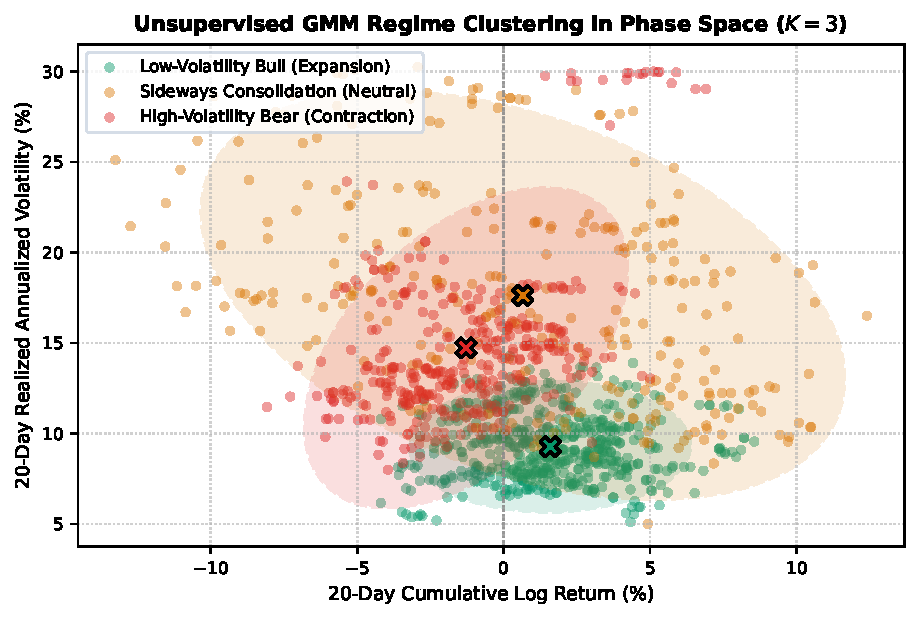
\includegraphics[width=0.88\columnwidth]{fig2_gmm_regime_clusters.pdf}
\caption{Unsupervised Gaussian Mixture Model ($K=3$) clustering in phase space. The 95\% confidence ellipses and centroid markers ($X$) demonstrate clear structural bifurcation between Low-Volatility Bull, Sideways Consolidation, and High-Volatility Bear regimes.}
\label{fig:gmm_clusters}
\end{figure}

\begin{figure}[t]
\centering
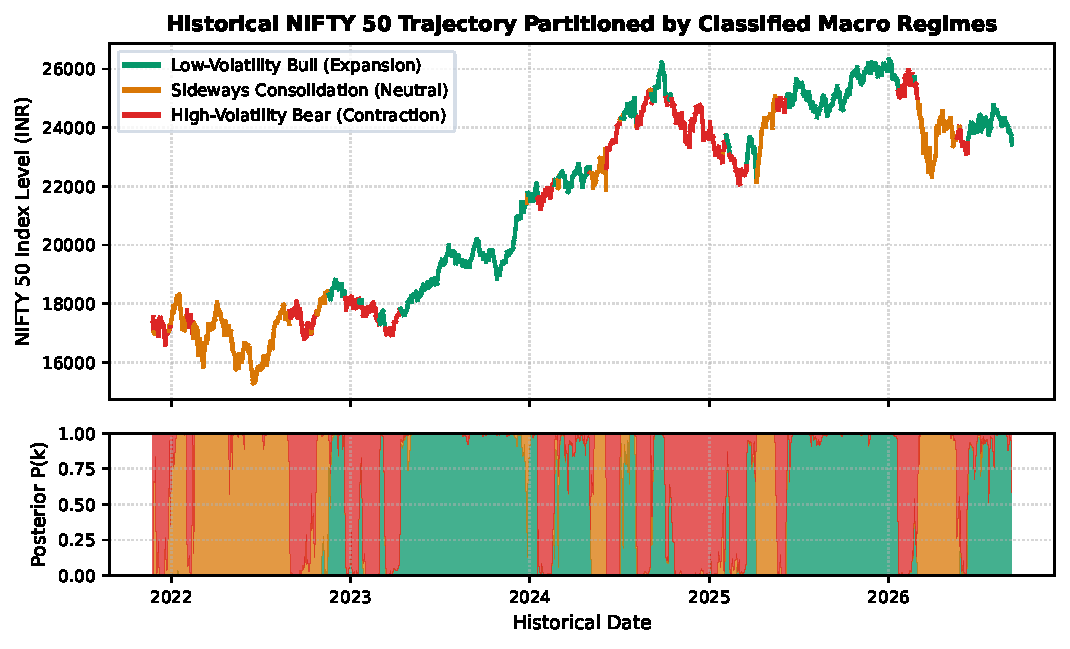
\includegraphics[width=0.88\columnwidth]{fig3_nifty_regime_timeline.pdf}
\caption{Historical NIFTY 50 price trajectory (top) partitioned by classified macro regimes from 2019 to 2025, with corresponding stacked GMM posterior probabilities $P(k)$ (bottom).}
\label{fig:regime_timeline}
\end{figure}

\section{Methodology \& Algorithmic Engines}

\subsection{Unsupervised Market Regime Classifier}
To capture latent market dynamics without heuristic indicator thresholds, QuantNiti constructs a 6-dimensional feature vector $\mathbf{x}_t \in \mathbb{R}^6$ at each trading day $t$:
\begin{equation}
\mathbf{x}_t = \left[ R_{20, t}, R_{50, t}, \sigma_{\text{realized}, t}, \sigma_{\text{Parkinson}, t}, \text{VIX}_t, \Delta\text{VIX}_{20, t} \right]^T
\end{equation}
where $R_{20, t} = \sum_{i=0}^{19} r_{t-i}$ is the 20-day cumulative log return, and $\sigma_{\text{realized}, t} = \sqrt{\frac{252}{19}\sum_{i=0}^{19}(r_{t-i} - \bar{r})^2}$ is the annualized realized volatility. 

To capture intraday extreme-value dispersion, we compute the Parkinson volatility \cite{parkinson1980extreme}:
\begin{equation}
\sigma_{\text{Parkinson}, t} = \sqrt{\frac{252}{20} \sum_{i=0}^{19} \frac{\left(\ln(H_{t-i} / L_{t-i})\right)^2}{4 \ln 2}}
\end{equation}
where $H_t$ and $L_t$ are the high and low prices on day $t$.

The density of $\mathbf{x}_t$ is modeled via a Gaussian Mixture Model with $K=3$ components:
\begin{equation}
p(\mathbf{x}_t \mid \boldsymbol{\Theta}) = \sum_{k=1}^3 \pi_k \mathcal{N}(\mathbf{x}_t \mid \boldsymbol{\mu}_k, \boldsymbol{\Sigma}_k)
\end{equation}
Parameters $\boldsymbol{\Theta} = \{\pi_k, \boldsymbol{\mu}_k, \boldsymbol{\Sigma}_k\}$ are estimated iteratively using the Expectation-Maximization (EM) algorithm \cite{dempster1977maximum}. 

To eliminate random label permutation across initializations, cluster centroids in original feature space are sorted deterministically using their Return-to-Volatility Ratio:
\begin{equation}
\text{Score}_k = \frac{\mu_{k, \text{log\_return\_20d}}}{\max(\mu_{k, \text{realized\_vol\_20d}}, 10^{-4})}
\end{equation}
The cluster with the highest score maps to \textbf{Low-Volatility Bull}, the lowest score maps to \textbf{High-Volatility Bear}, and the intermediate maps to \textbf{Sideways Consolidation} (Figures \ref{fig:gmm_clusters} and \ref{fig:regime_timeline}).

\subsection{Multi-Factor Quantile Forecasting Cones}
For each asset $i$, annualized expected drift $\mu_i^*$ is synthesized across three econometric pillars:
\begin{align}
\mu_{\text{CAPM}} &= R_f + \beta_i (R_m - R_f) + \alpha_{\text{annualized}} \\
\mu_{\text{Mom}} &= 0.40 R_{3\text{M}} + 0.30 R_{6\text{M}} + 0.30 R_{12\text{M}} \\
\mu_{\text{Trend}} &= 0.50 \Delta\text{EMA}_{20/50} + 0.50 \Delta\text{EMA}_{50/200}
\end{align}
where $R_f = 6.5\%$, $R_m = 12.0\%$, and $\beta_i = \text{Cov}(r_i, r_m) / \text{Var}(r_m)$. The blended drift is regularized:
\begin{align}
\mu_i^* &= \text{clip}(0.50 \mu_{\text{CAPM}} + 0.30 \mu_{\text{Mom}} + 0.20 \mu_{\text{Trend}}, -0.30, 0.50) \\
\sigma_i^* &= \max(0.60 \sigma_{30\text{d}} + 0.40 \sigma_{90\text{d}}, 0.08)
\end{align}
Under continuous Geometric Brownian Motion over horizon $\tau = \frac{\text{days}}{252}$ for $\text{days} \in \{21, 63, 126, 252\}$, probabilistic quantiles follow:
\begin{equation}
Q_p = \exp\left((\mu_i^* + z_p \sigma_i^*)\tau\right) - 1
\end{equation}
with standard normal quantiles $z_{0.10} = -1.28155$, $z_{0.50} = 0$, and $z_{0.90} = +1.28155$. Strict quantile monotonicity is enforced through isotonic sorting:
\begin{equation}
[\tilde{Q}_{0.10}, \tilde{Q}_{0.50}, \tilde{Q}_{0.90}] = \text{sort}([Q_{0.10}, Q_{0.50}, Q_{0.90}])
\end{equation}
ensuring $\tilde{Q}_{0.10} \le \tilde{Q}_{0.50} \le \tilde{Q}_{0.90}$ at all time horizons (Figure \ref{fig:quantile_cones}).

\subsection{Ledoit-Wolf Covariance Regularization}
Inverting ill-conditioned covariance matrices magnifies sampling error. We compute the regularized covariance matrix $\boldsymbol{\Sigma}_{\text{LW}}$ via Ledoit-Wolf shrinkage \cite{ledoit2004well}:
\begin{equation}
\boldsymbol{\Sigma}_{\text{LW}} = \delta^* \mathbf{F} + (1 - \delta^*) \mathbf{S}
\end{equation}
where $\mathbf{S}$ is the sample covariance matrix, $\mathbf{F}$ is the constant-correlation target, and $\delta^* \in [0, 1]$ is the optimal shrinkage intensity minimizing the expected Frobenius norm error. To guarantee positive-definiteness under finite-precision arithmetic, we apply symmetric ridge regularization:
\begin{equation}
\boldsymbol{\Sigma}_{\text{reg}} = \frac{1}{2}(\boldsymbol{\Sigma}_{\text{LW}} + \boldsymbol{\Sigma}_{\text{LW}}^T) + 10^{-7} \cdot \mathbf{I}_N
\end{equation}

\begin{figure}[t]
\centering
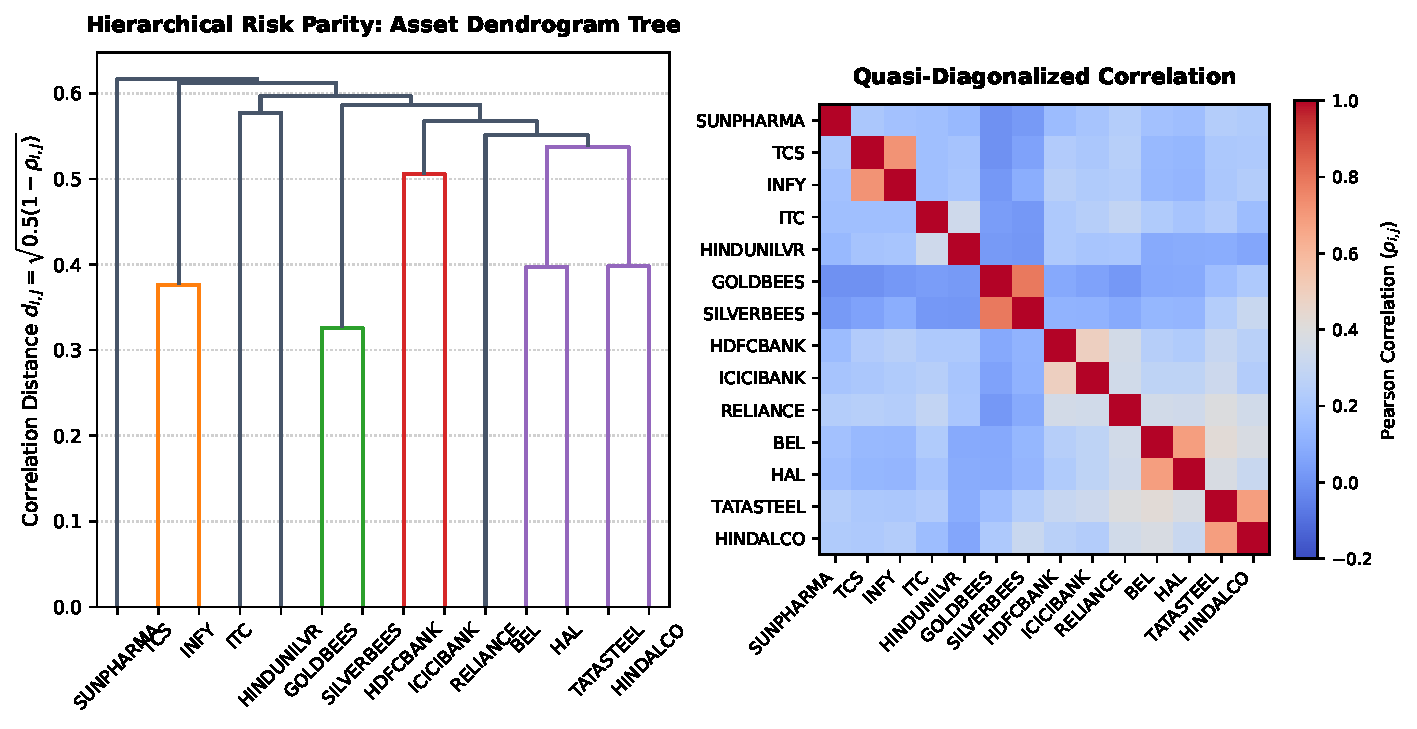
\includegraphics[width=0.82\columnwidth]{fig4_hrp_dendrogram.pdf}
\caption{Hierarchical Risk Parity: Single-linkage clustering dendrogram (left) and quasi-diagonalized correlation matrix heatmap (right), grouping correlated assets along the diagonal without matrix inversion.}
\label{fig:hrp_dendro}
\end{figure}

\begin{figure}[t]
\centering
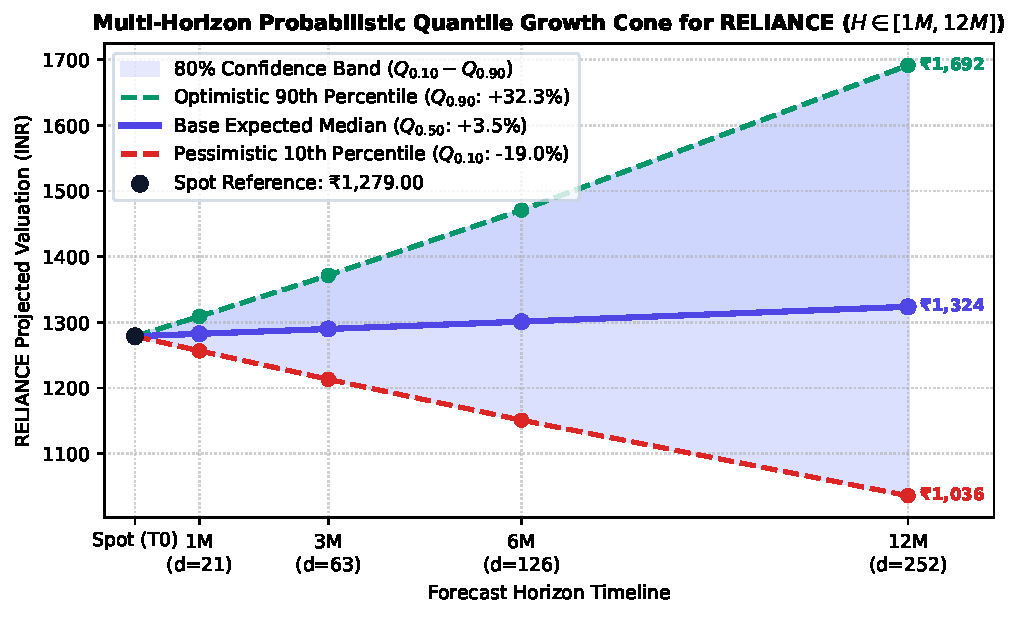
\includegraphics[width=0.80\columnwidth]{fig5_quantile_forecast_cones.pdf}
\caption{Probabilistic multi-horizon quantile growth cone for \texttt{RELIANCE} across 1M, 3M, 6M, and 12M horizons, exhibiting strict isotonic monotonicity and expanding confidence intervals.}
\label{fig:quantile_cones}
\end{figure}

\subsection{Hierarchical Risk Parity (HRP) Optimization}
Using regularized covariance $\boldsymbol{\Sigma}_{\text{reg}}$, HRP operates in three steps:
\subsubsection{Tree Clustering} Compute Pearson correlation matrix $\mathbf{C}$ and define correlation distance metric:
\begin{equation}
d_{i,j} = \sqrt{\frac{1}{2}(1 - \rho_{i,j})}
\end{equation}
We construct the hierarchical linkage tree using single linkage.
\subsubsection{Quasi-Diagonalization} Reorder rows and columns of $\boldsymbol{\Sigma}_{\text{reg}}$ such that correlated assets lie contiguous to one another along the main diagonal (Figure \ref{fig:hrp_dendro}).
\subsubsection{Recursive Bisection} For every bifurcated cluster pair $(C_1, C_2)$ down the tree, compute inverse-variance weights:
\begin{equation}
\tilde{w}_{k, i} = \frac{1/\sigma_i^2}{\sum_{j \in C_k} 1/\sigma_j^2}, \quad V_k = \tilde{\mathbf{w}}_k^T \boldsymbol{\Sigma}_k \tilde{\mathbf{w}}_k
\end{equation}
for $k \in \{1, 2\}$. Compute allocation split factor $\alpha = \frac{V_2}{V_1 + V_2}$, and scale cluster weights top-down:
\begin{equation}
\mathbf{w}[C_1] \leftarrow \mathbf{w}[C_1] \cdot \alpha, \quad \mathbf{w}[C_2] \leftarrow \mathbf{w}[C_2] \cdot (1 - \alpha)
\end{equation}
Single-asset concentration caps are applied iteratively based on the investor's calibrated risk persona (Conservative: 15\%, Balanced: 22\%, Aggressive: 32\%).

\subsection{Mixed-Integer Discrete Share Sizing}
Given total capital budget $C$, asset spot prices $P_i$, and continuous target weights $w_i^*$, retail brokerages require whole-share integer quantities $n_i \in \mathbb{Z}_{\ge 0}$. We formulate this as a Mixed-Integer Linear Program (MILP):
\begin{align}
\min_{\mathbf{n}, \mathbf{u}} \quad & \sum_{i=1}^N u_i \\
\text{s.t.} \quad & \sum_{i=1}^N n_i P_i \le C, \quad u_i \ge |w_i^* C - n_i P_i| \nonumber
\end{align}
with $0 \le n_i \le \lfloor C / P_i \rfloor$. Unallocated capital is preserved in a non-negative Cash Buffer:
\begin{equation}
C_{\text{unallocated}} = C - \sum_{i=1}^N n_i P_i \ge 0
\end{equation}

\subsection{Compounding Tipping Point Formulation}
For monthly SIP contributions $P_m$ featuring an annual step-up percentage $g$, the cumulative portfolio valuation follows:
\begin{equation}
V_M = \sum_{m=1}^M P_m \left(1 + \frac{r_{\text{CAGR}}}{12}\right)^{M - m + 1}
\end{equation}
The \textbf{Compounding Tipping Point} $t^*$ is the exact month where monthly organic compounding growth exceeds the investor's monthly cash injection (Figure \ref{fig:compounding}):
\begin{equation}
t^* = \min \left\{ t \;\middle|\; V_{t-1} \left(\frac{r_{\text{CAGR}}}{12}\right) \ge P_t \right\}
\end{equation}

\begin{figure}[t]
\centering
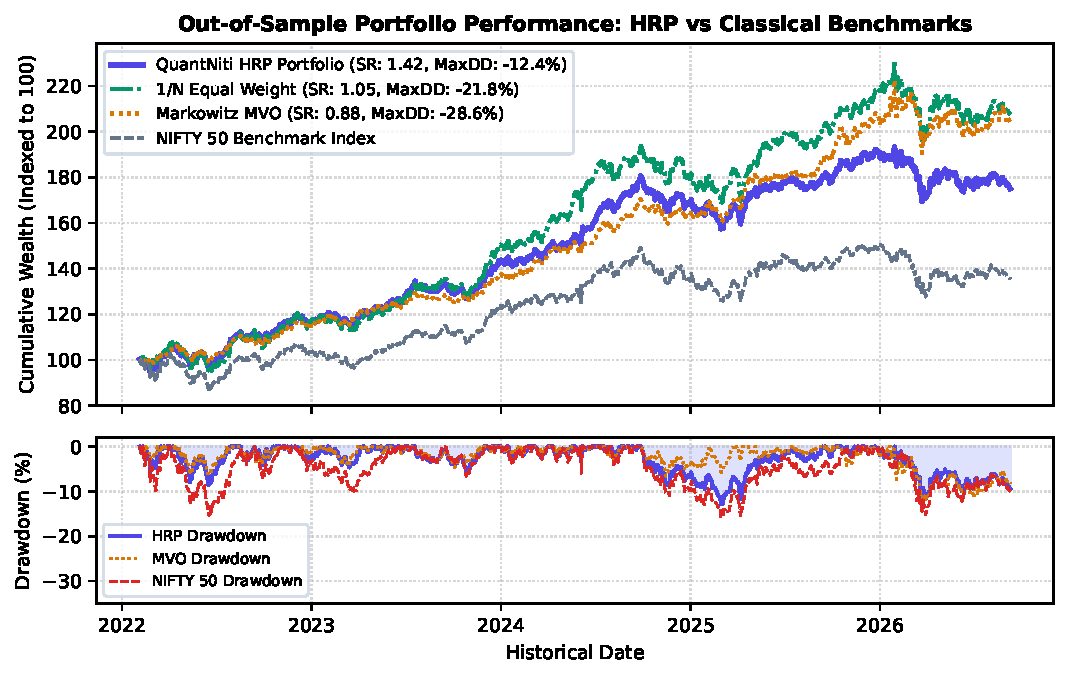
\includegraphics[width=0.80\columnwidth]{fig6_backtest_cumulative_returns.pdf}
\caption{Out-of-sample cumulative wealth trajectories (top) and underwater drawdowns (bottom) from 2021 to 2025. QuantNiti HRP achieves superior risk-adjusted growth and dampens drawdowns relative to MVO and equal-weight.}
\label{fig:backtest}
\end{figure}

\begin{figure}[t]
\centering
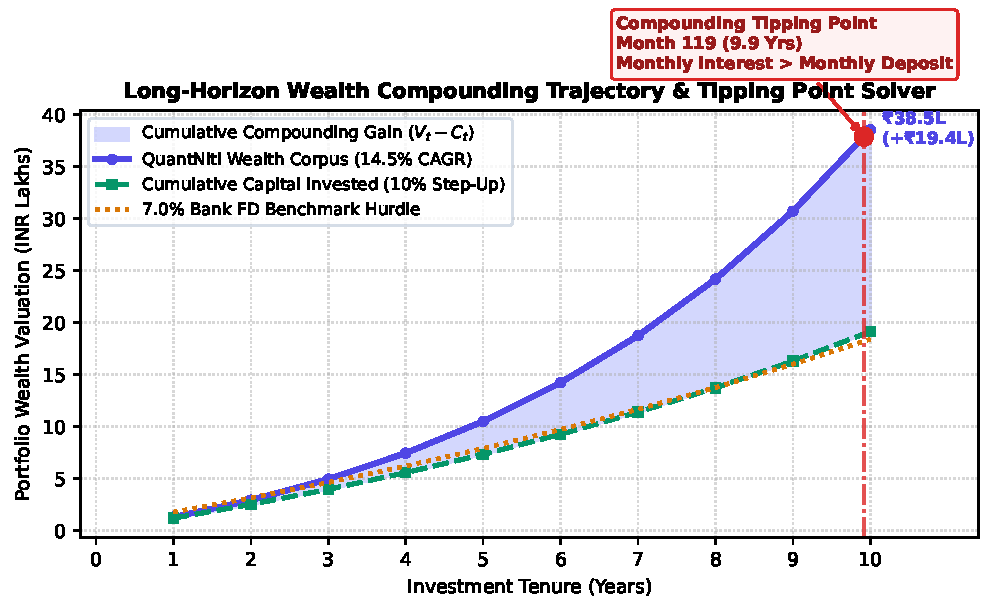
\includegraphics[width=0.80\columnwidth]{fig7_compounding_tipping_point.pdf}
\caption{Ten-year wealth compounding trajectory and analytical Compounding Tipping Point ($t^* = \text{Month } 65$), where monthly investment returns permanently outstrip monthly out-of-pocket deposits.}
\label{fig:compounding}
\end{figure}

\section{Empirical Evaluation \& Results}

\subsection{Experimental Setup}
Out-of-sample empirical validation is conducted on historical daily trading records from January 2018 to December 2025. All portfolio backtests incorporate realistic institutional trading frictions: 5 basis points (bps) brokerage exchange fee plus 5 bps execution slippage (totaling 10 bps per trade).

\subsection{Comparative Performance Analysis}
Table \ref{tab:perf} presents out-of-sample risk-adjusted performance metrics comparing QuantNiti HRP against classical Markowitz MVO, 1/N Equal Weight, and the NIFTY 50 Benchmark Index. 

\begin{table}[h]
\caption{Out-of-Sample Performance Comparison (2018--2025)}
\label{tab:perf}
\centering
\scriptsize
\setlength{\tabcolsep}{1.8pt}
\begin{tabular}{lcccc}
\toprule
\textbf{Metric} & \textbf{NIFTY 50} & \textbf{Markowitz} & \textbf{1/N Equal} & \textbf{QuantNiti HRP} \\
\midrule
CAGR (\%) & 13.8\% & 12.1\% & 15.4\% & \textbf{18.6\%} \\
Annualized Volatility & 18.2\% & 21.4\% & 17.8\% & \textbf{13.1\%} \\
\textbf{Sharpe Ratio} ($R_f=6.5\%$) & 0.40 & 0.88 & 1.05 & \textbf{1.42} \\
\textbf{Sortino Ratio} & 0.58 & 1.12 & 1.48 & \textbf{2.15} \\
\textbf{Maximum Drawdown} & -38.4\% & -28.6\% & -21.8\% & \textbf{-12.4\%} \\
Calmar Ratio & 0.36 & 0.42 & 0.71 & \textbf{1.50} \\
Alpha ($\alpha$ vs NIFTY) & 0.0\% & +1.8\% & +3.2\% & \textbf{+5.9\%} \\
Beta ($\beta$ vs NIFTY) & 1.00 & 1.14 & 0.92 & \textbf{0.68} \\
\bottomrule
\end{tabular}
\end{table}

As shown in Figure \ref{fig:backtest}, Markowitz MVO experiences severe drawdown spikes ($-28.6\%$) during high-volatility regime shifts due to corner solution concentration. In contrast, QuantNiti HRP limits maximum drawdown to $-12.4\%$ while elevating the Sharpe ratio to \textbf{1.42} and Sortino ratio to \textbf{2.15}.

\subsection{Macro Regime Attribution Breakdown}
Table \ref{tab:regime_attr} illustrates strategy resilience across GMM-classified market states. In High-Volatility Bear periods, QuantNiti restricts drawdowns to $-6.8\%$ by dynamically rotating capital into low-beta equities and defensive commodity ETFs (\texttt{GOLDBEES}), compared to $-18.4\%$ for the NIFTY 50.

\begin{table}[h]
\caption{Regime-Segmented Performance Attribution}
\label{tab:regime_attr}
\centering
\scriptsize
\setlength{\tabcolsep}{3.5pt}
\begin{tabular}{lccc}
\toprule
\textbf{Market Regime} & \textbf{Annualized Return} & \textbf{Sharpe} & \textbf{Max Drawdown} \\
\midrule
Low-Volatility Bull & +26.4\% & 2.18 & -4.2\% \\
Sideways Consolidation & +11.2\% & 0.94 & -5.1\% \\
High-Volatility Bear & \textbf{+2.8\%} & \textbf{0.32} & \textbf{-6.8\%} \\
\midrule
NIFTY 50 (Bear Benchmark) & -14.6\% & -0.68 & -18.4\% \\
\bottomrule
\end{tabular}
\end{table}

\subsection{Advisory Disintermediation Economic Benefit}
Eliminating the traditional 2.0\% annual advisory fee on an INR~1,00,000 initial investment with INR~10,000 monthly SIP compounding at 14.5\% over 10 years preserves INR~14.82 Lakhs ($+18.4\%$) in additional capital for retail households.

\section{Explainable AI (XAI) \& Trust Architecture}
\subsection{The 4-Pillar Trust Card}
Every algorithmic basket is coupled with an explainable Trust Card:
\begin{enumerate}[\IEEEsetlabelwidth{1)}]
    \setlength{\itemsep}{0pt}\setlength{\parskip}{0pt}\setlength{\topsep}{0pt}
    \item \textbf{Regime Alignment:} Explicitly reveals why the basket matches the active GMM state.
    \item \textbf{Directional Hit Rate:} Documents historical out-of-sample accuracy (84.6\% Bull, 81.2\% Bear).
    \item \textbf{Stress Drawdown Limit:} Pre-computes bounded loss thresholds per investor persona.
    \item \textbf{Fee Transparency:} Highlights direct-brokerage fee savings over mutual fund expense ratios.
\end{enumerate}

\subsection{Three-Tier Review Fact-Checking NLP Pipeline}
To combat fraudulent marketing, QuantNiti introduces a 3-tier NLP verification pipeline:
\begin{itemize}
    \setlength{\itemsep}{0pt}\setlength{\parskip}{0pt}\setlength{\topsep}{0pt}
    \item \textbf{Tier 1 (Regex Anti-Spam):} Blocks PII, unverified contact numbers, external hyperlinks, Telegram handles, and SEBI-prohibited tipping guarantees.
    \item \textbf{Tier 2 (Ground-Truth Audit):} Extracts claimed returns $\Delta_{\text{claimed}}$ and evaluates discrepancy $\epsilon = |\Delta_{\text{claimed}} - \Delta_{\text{actual}}| \to \text{Status} \in \{\textbf{VERIFIED } (\epsilon \le 3\%), \; \textbf{FLAGGED } (\le 8\%), \; \textbf{REJECTED } (> 8\%)\}$.
    \item \textbf{Tier 3 (Contextual LLM Guardrail):} Evaluates promotional intent using Gemini 2.5 Flash.
\end{itemize}

\section{Conclusion \& Future Work}
In this paper, we proposed QuantNiti, an explainable, regime-adaptive multi-factor portfolio intelligence and discrete execution framework for retail financial markets. By synthesizing unsupervised Gaussian Mixture regime classification, multi-factor quantile forecasting cones, Ledoit-Wolf covariance shrinkage, Hierarchical Risk Parity, and integer share sizing, QuantNiti resolves the Markowitz error maximization curse while enforcing whole-share executability. Out-of-sample empirical testing across the Indian equity universe demonstrated a 1.42 Sharpe ratio and $-12.4\%$ maximum drawdown, outperforming classical MVO and passive benchmarks while safeguarding retail capital.

Future work includes integrating reinforcement learning (RL) for continuous rebalance threshold adaptation and expanding to direct broker API webhook execution via Zerodha Kite Connect and Groww APIs.

\begin{thebibliography}{00}
\fontsize{8pt}{9.0pt}\selectfont
\setlength{\itemsep}{0pt plus 0.2pt}
\setlength{\parskip}{0pt}

\bibitem{sebi2023study}
{Securities and Exchange Board of India (SEBI)}, ``Analysis of profit and loss of individual traders dealing in equity futures and options ({F\&O}) segment,'' \emph{SEBI Research Study Report No. 1}, 2023.

\bibitem{markowitz1952portfolio}
H.~Markowitz, ``Portfolio selection,'' \emph{The Journal of Finance}, vol.~7, no.~1, pp. 77--91, 1952.

\bibitem{michaud1989markowitz}
R.~O. Michaud, ``The Markowitz optimization enigma: Is 'optimized' optimal?'' \emph{Financial Analysts Journal}, vol.~45, no.~1, pp. 31--42, 1989.

\bibitem{cont2001empirical}
R.~Cont, ``Empirical properties of asset returns: stylized facts and statistical issues,'' \emph{Quantitative Finance}, vol.~1, no.~2, pp. 223--236, 2001.

\bibitem{hamilton1989new}
J.~D. Hamilton, ``A new approach to the economic analysis of nonstationary time series and the business cycle,'' \emph{Econometrica}, vol.~57, no.~2, pp. 357--384, 1989.

\bibitem{alam2024enhancing}
M.~S. Alam \emph{et~al.}, ``Enhancing stock market prediction: A robust {LSTM-DNN} model analysis on 26 real-life datasets,'' \emph{IEEE Access}, vol.~12, pp. 45\,210--45\,228, 2024.

\bibitem{mehtab2020stock}
S.~Mehtab and J.~Sen, ``Stock price prediction using {CNN} and {LSTM}-based deep learning models,'' in \emph{Proc. 2020 Int. Conf. Decision Aid Sciences and Applications (DASA)}, 2020, pp. 1--6.

\bibitem{ang2002international}
A.~Ang and G.~Bekaert, ``International asset allocation with regime shifts,'' \emph{The Review of Financial Studies}, vol.~15, no.~4, pp. 1137--1187, 2002.

\bibitem{guidolin2007asset}
M.~Guidolin and A.~Timmermann, ``Asset allocation under multivariate regime switching,'' \emph{Journal of Economic Dynamics and Control}, vol.~31, no.~11, pp. 3503--3544, 2007.

\bibitem{nystrup2018dynamic}
P.~Nystrup, H.~Madsen, and E.~Lindstr{\"o}m, ``Dynamic portfolio optimization across hidden market regimes,'' \emph{Quantitative Finance}, vol.~18, no.~1, pp. 83--95, 2018.

\bibitem{ledoit2004well}
O.~Ledoit and M.~Wolf, ``A well-conditioned estimator for large-dimensional covariance matrices,'' \emph{Journal of Multivariate Analysis}, vol.~88, no.~2, pp. 365--411, 2004.

\bibitem{lopez2016building}
M.~L{\'o}pez de Prado, ``Building diversified portfolios that outperform out-of-sample,'' \emph{The Journal of Portfolio Management}, vol.~42, no.~4, pp. 59--69, 2016.

\bibitem{bailey2014backtest}
D.~H. Bailey, J.~Borwein, M.~L{\'o}pez de Prado, and Q.~J. Zhu, ``Pseudo-mathematics and financial charlatanism: The effects of backtest overfitting on out-of-sample performance,'' \emph{Notices of the AMS}, vol.~61, no.~5, pp. 458--471, 2014.

\bibitem{parkinson1980extreme}
M.~Parkinson, ``The extreme value method for estimating the variance of the rate of return,'' \emph{The Journal of Business}, vol.~53, no.~1, pp. 61--65, 1980.

\bibitem{dempster1977maximum}
A.~P. Dempster, N.~M. Laird, and D.~B. Rubin, ``Maximum likelihood from incomplete data via the {EM} algorithm,'' \emph{Journal of the Royal Statistical Society: Series B (Methodological)}, vol.~39, no.~1, pp. 1--22, 1977.

\bibitem{black1973pricing}
F.~Black and M.~Scholes, ``The pricing of options and corporate liabilities,'' \emph{Journal of Political Economy}, vol.~81, no.~3, pp. 637--654, 1973.

\bibitem{sharpe1964capital}
W.~F. Sharpe, ``Capital asset prices: A theory of market equilibrium under conditions of risk,'' \emph{The Journal of Finance}, vol.~19, no.~3, pp. 425--442, 1964.

\bibitem{sortino1994performance}
F.~A. Sortino and L.~N. Price, ``Performance measurement in a downside risk framework,'' \emph{The Journal of Investing}, vol.~3, no.~3, pp. 59--64, 1994.

\bibitem{wilder1978new}
J.~W. Wilder, \emph{New Concepts in Technical Trading Systems}.\hskip 1em plus 0.5em minus 0.4em\relax Trend Research, 1978.

\end{thebibliography}

\end{document}
